\documentclass{article}


\usepackage{circuitikz} %Für die Schaltpläne
\usepackage[T1]{fontenc}
\usepackage[utf8]{inputenc}
\usepackage{amsmath}
\usepackage{amssymb}
\usepackage{fancyhdr}
\usepackage{graphicx}
\usepackage{hyperref}
\usepackage{subcaption}
\usepackage{tikz}
\usepackage{cite}
\usepackage[nottoc, numbib]{tocbibind}
\usepackage{../assets/scripts/tex/color-env}
\usepackage[ngerman]{babel}



    \usetikzlibrary{arrows}
    \usetikzlibrary{arrows.meta,topaths}
    \usetikzlibrary{bending}
    \usetikzlibrary{calc}
\title{Elektrotechnik 1 Praktikum 1}


\usepackage[
  includehead,
  headheight = 17mm,
  footskip = \dimexpr\headsep+\ht\strutbox\relax,
  tmargin = 0mm,
  bmargin = \dimexpr17mm+2\ht\strutbox\relax,
]{geometry}

\usepackage{anyfontsize}

\usepackage{xcolor}

\definecolor{DarkGreenBlue}{HTML}{264653}
\definecolor{LightGreenBlue}{HTML}{2A9D8F}
\definecolor{LightOrange}{HTML}{E9C46A}
\definecolor{DarkOrange}{HTML}{F4A261}
\definecolor{RedOrange}{HTML}{E76F51}
\definecolor{BrightRed}{HTML}{D62828}
\definecolor{DeepBlue}{HTML}{003049}



\pagestyle{fancy}
\fancyhead[L]{\leftmark}
\fancyhead[R]{}
\fancyfoot[L]{}
\fancyfoot[C]{\thepage}
\fancyfoot[R]{
\includegraphics[scale=0.2]{../assets/images/haw.jpg}}
\renewcommand\headrulewidth{0.5pt}


\begin{document}



\begin{tikzpicture}[overlay,remember picture]
  \thispagestyle{empty}
  \fill[black!2] (current page.south west) rectangle (current page.north east);

  \begin{scope}[transform canvas ={rotate around ={45:($(current page.north west)+(-.5,-6)$)}}]

    \shade[rounded corners=18pt, left color=DarkGreenBlue, right color=LightGreenBlue] ($(current page.north west)+(-.5,-6)$) rectangle ++(9,1.5);

  \end{scope}

  \begin{scope}[transform canvas ={rotate around ={45:($(current page.north west)+(.5,-10)$)}}]

    \shade[rounded corners=18pt, left color=LightOrange,right color=DarkOrange] ($(current page.north west)+(0.5,-10)$) rectangle ++(15,1.5);

  \end{scope}

  \begin{scope}[transform canvas ={rotate around ={45:($(current page.north west)+(0.5,-10)$)}}]

    \shade[rounded corners=8pt, right color=DarkOrange, left color=LightOrange] ($(current page.north west)+(1.5,-9.55)$) rectangle ++(7,.6);

  \end{scope}

  \begin{scope}[transform canvas ={rotate around ={45:($(current page.north)+(-1.5,-3)$)}}]

    \shade[rounded corners=12pt, left color=DeepBlue!80, right color=DeepBlue!60] ($(current page.north)+(-1.5,-3)$) rectangle ++(9,0.8);

  \end{scope}

  \begin{scope}[transform canvas ={rotate around ={45:($(current page.north)+(-3,-8)$)}}]

    \shade[rounded corners=28pt, left color=BrightRed, right color=BrightRed!80] ($(current page.north)+(-3,-8)$) rectangle ++(15,1.8);

  \end{scope}

  \begin{scope}[transform canvas ={rotate around ={45:($(current page.north west)+(4,-15.5)$)}}]

    \shade[rounded corners=25pt, left color=RedOrange, right color=DarkOrange] ($(current page.north west)+(4,-15.5)$) rectangle ++(30,1.8);

  \end{scope}

  \begin{scope}[transform canvas ={rotate around ={45:($(current page.north west)+(13,-10)$)}},]

    \shade[rounded corners=22pt, left color=DeepBlue,right color=DarkGreenBlue] ($(current page.north west)+(13,-10)$) rectangle ++(15,1.5);

  \end{scope}

  \begin{scope}[transform canvas ={rotate around ={45:($(current page.north west)+(18,-8)$)}},]

    \shade[rounded corners=8pt, left color=DarkOrange] ($(current page.north west)+(18,-8)$) rectangle ++(15,0.6);

  \end{scope}

  \begin{scope}[transform canvas ={rotate around ={45:($(current page.north west)+(19,-5.65)$)}},]

    \shade[rounded corners=12pt, left color=RedOrange] ($(current page.north west)+(19,-5.65)$) rectangle ++(15,0.8);

  \end{scope}

  \begin{scope}[transform canvas ={rotate around ={45:($(current page.north west)+(20,-9)$)}}]

    \shade[rounded corners=20pt, left color=BrightRed, right color=BrightRed!80] ($(current page.north west)+(20,-9)$) rectangle ++(14,1.2);

  \end{scope}

  \draw[ultra thick,gray] ($(current page.center)+(5,2)$) -- ++(0,-3cm) node[midway,left=0.25cm,text width=5cm,align=right,black!75]{{\fontsize{25}{30} \selectfont \bf Elektronik 2\\[10pt] Praktikum 1}} node[midway,right=0.25cm,text width=6cm,align=left,orange]{{\fontsize{70}{86} \selectfont 2021}};

  \node at ($(current page.center)+(0,-4)$) {{\fontsize{60}{72} \selectfont Differenzverstärker}};

  \node[text width=8cm,align=center] at ($(current page.center)+(0,-6.5)$) {{\fontsize{16}{20} \selectfont \textcolor{orange}{ \bf \today}} \\[3pt] Florian Tietjen\\[3pt] Torsten Möller\\[3pt] Eric Antosch};

\end{tikzpicture}
\newpage
\thispagestyle{empty}

\tableofcontents

\listoffigures
\newpage


\section{Grundschaltung eines Differenzverstärkers}
\begin{task}
  TBei dieser Aufgabe soll die Grundschaltung eines Differenzverstärkers mit zwei BC546B-Transistoren mit beiden Basen an GND beschrieben werden.
\end{task}

\begin{figure}[h]
  \centering
  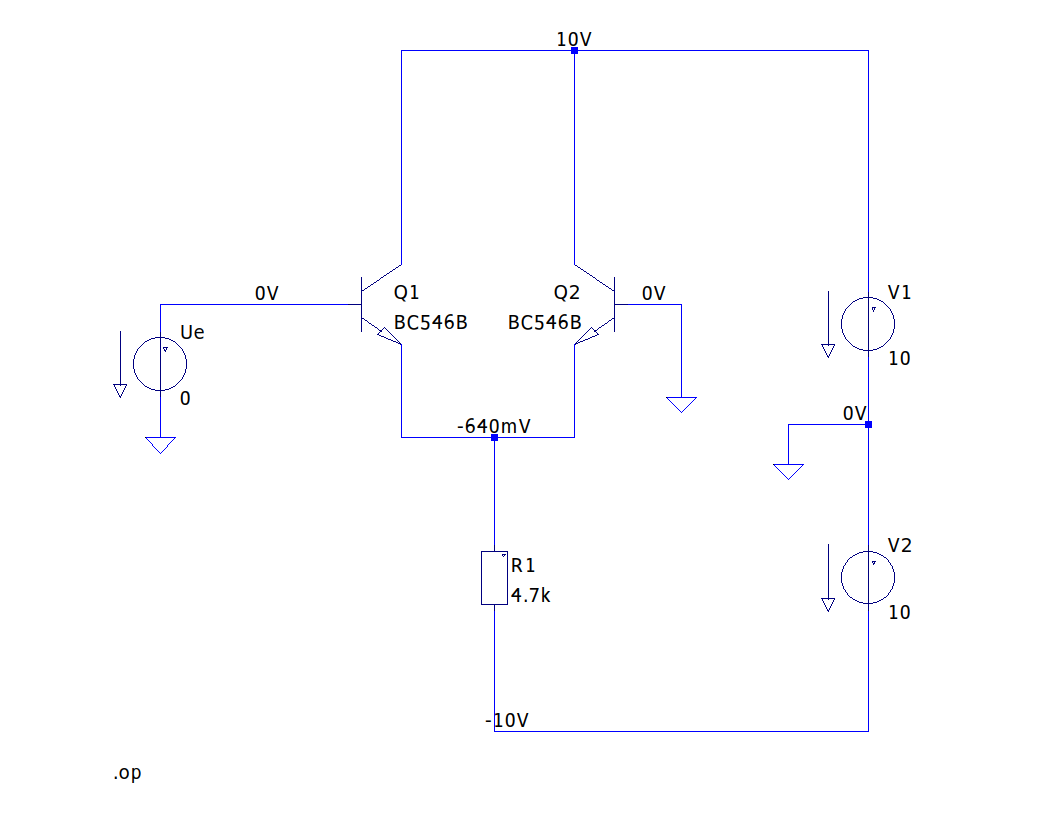
\includegraphics[scale=0.5]{../assets/images/EL2P1/aufgabe1schalt.png}
  \caption[Grundschaltung der Differenzverstärker]{Grundschaltung eines Differenzverstärkers}
  \label{fig:schalt1}
\end{figure}

\subsection{Dimensionierung des $R_E$-Widerstands}
\label{sec:RE}

Wir wollen nun zunächst unseren $R_E$-Widerstand mithilfe der gegebenen Formeln \cite{skript} berechnen:
\begin{equation}
 R_E = \frac{U_B-U_{BE}}{2\cdot I_C}
\end{equation}

Wir erhalten mit dem Einsetzen der Werte für $I_C = 1mA$, $U_B = 10V$ und $U_{BE} = 0,7V$ ungefähr
einen Widerstandswert von $R_E = 4650\Omega$. Da unser Widerstand $R_E$ aus der E12-Reihe sein soll,
wählen wir mit $4700\Omega$ den passenden Widerstandswert.
\newpage

\section{Differenzverstärkung \textorpdfstring{$H_{D}$}}

\begin{task}
  TIn dieser Aufgabe wollen wir die Differenzverstärkung unserer Grundschaltung ermitteln, indem wir den linken Transistor nun von einer Spannungsquelle
  ansteuern lassen.
\end{task}

\begin{figure}[h]
  \centering
  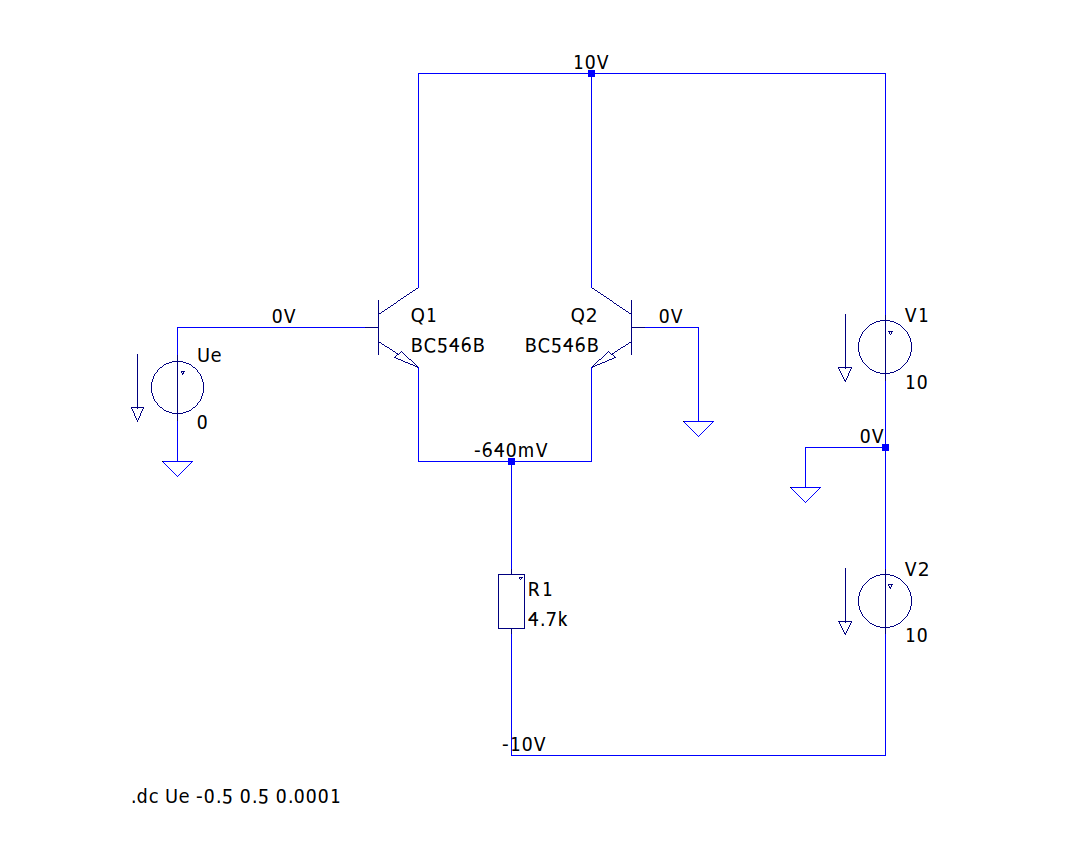
\includegraphics[scale=0.5]{../assets/images/EL2P1/aufgabe2schalt.png}
  \caption{Versuchsaufbau}
  \label{fig:schalt2}
\end{figure}

Wir nutzen nun die DC-Sweep-Analyse von LTSpice um die Spannung der Ue-Quelle linear von $-0,5V$ bis $0,5V$
wachsen zu lassen. Aus der Vorlesung kennen wir die Bedeutung von $U_d$, welches die Differenz der
Potentiale an den Basen der beiden Transistoren darstellt.\cite{skript}

\begin{equation}
  I_{C_{1}} = \frac{2\cdot I_{0}}{1+e^{-\frac{U_{d}}{U_{T}}}}
\end{equation}

\begin{equation}
  \label{eq:10}
  I_{C_{2}} = \frac{2\cdot I_{0}}{1+e^{+\frac{U_{d}}{U_{T}}}}
\end{equation}
\newpage
Tragen wir nun die Ströme durch die beiden Transistoren gegen die Differenzspannung $U_d$ ab, so
entsteht folgendes Bild:

\begin{figure}[h]
  \centering
  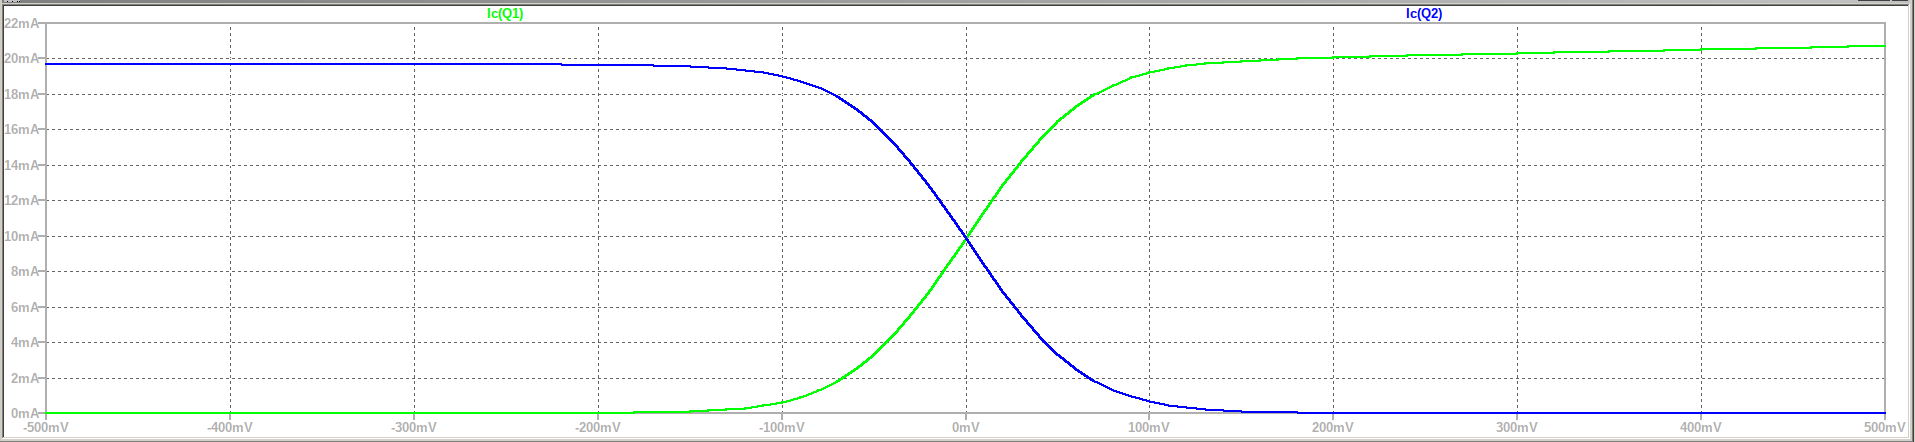
\includegraphics[scale=0.3]{../assets/images/EL2P1/DeepinScreenshot_select-area_20210417230438.png}
  \caption{Darstellung der Kollektorströme gegen die Differenzspannung $U_d$}
\end{figure}

Wir erkennen sowohl eine ziemlich genaue Übereinstimmung der Diagramme aus der Vorlesung als auch aus den
Praktikumsaufgaben.
Bei einer Differenzspannung von $U_d = 0V$ erhalten wir zudem unsere $I_C = 1 mA$, die wir in Aufgabe 1 bereits
verwendet haben. \\
Wir wollen nun noch einmal die Steilheit der Schaltung im Arbeitspunkt berechnen. Dafür legen wir bei dem Punkt $U_{d} = 0V$ ein Steigungsdreieck an, da:
\begin{equation}
  \label{eq:11}
  S_{1,2} = \pm\frac{dI_{C_{1,2}}}{dU_{d}}
\end{equation}

\begin{figure}[h]
  \centering
  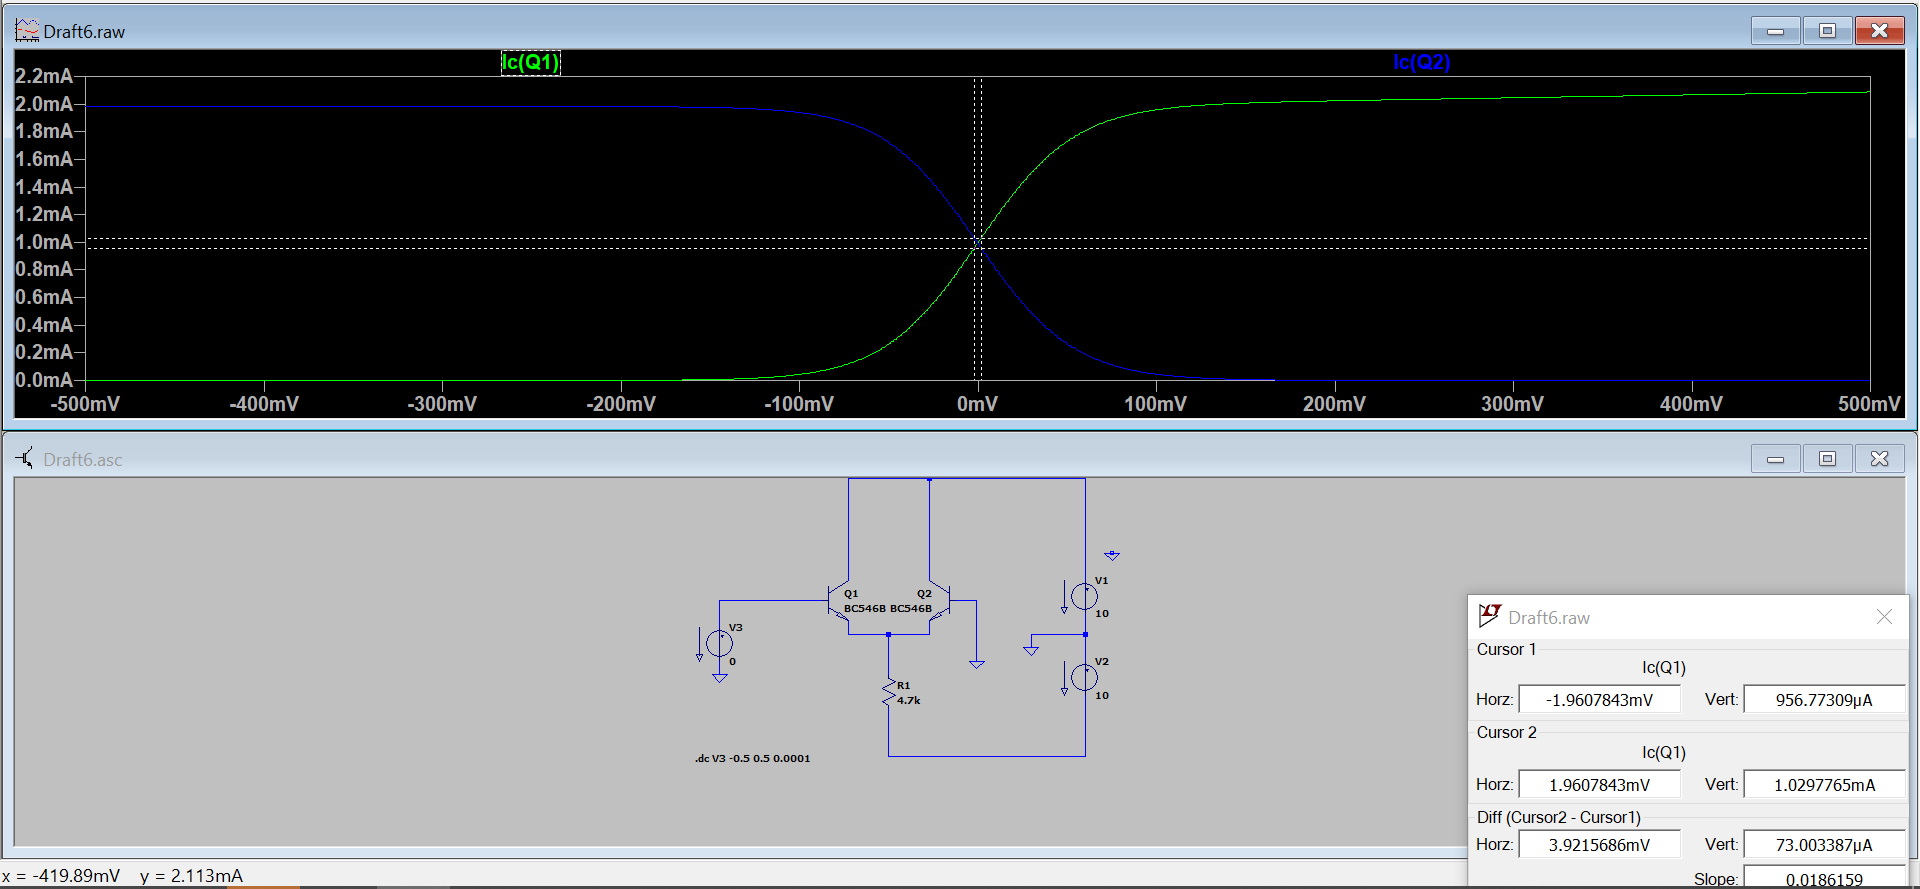
\includegraphics[scale=0.5]{../assets/images/EL2P1/aufgabe2slope.png}
  \caption{Anlegung der Cursor an die entsprechenden Punkte (siehe Slope)}
  \label{fig:diag2}
\end{figure}

Wie auf dem Bild unten links zu erkennen ist, bekommen wir eine Steigung von ungefähr $S_{1,2}=\pm 0,0186 \frac{A}{V}$.
Berechnen wir mithilfe der aus der Vorlesung gegebenen Formel, so ergibt sich\cite{skript}:
\begin{equation}
  \label{eq:12}
  S_{1,2} = \pm \frac{I_{C_{0}}}{2\cdot U_{T}} =\pm 0,02 \frac{A}{V}
\end{equation}
Die Werte liegen also, wie sich leicht erkennen lässt, nicht weit auseinander und die Abweichung ist wahrscheinlich durch Ungenauigkeiten beim Messen oder durch Rundungen beim Rechnen entstanden.
\newpage


\section{Gegen- und Gleichtaktverstärkung}

\begin{task}
TNun werden in den Kollektorzweigen der Transistoren Widerstände $R_{C1}$ und $R_{C2}$ von jeweils $1k\Omega$ ergänzt. Ziel des Versuchs ist die Untersuchung der Gegen- und Gleichtaktverstärkung sowie der Vergleich der Messergebnisse mit den theoretischen Berechnungen.
\end{task}

\begin{figure}[h]
  \begin{center}
    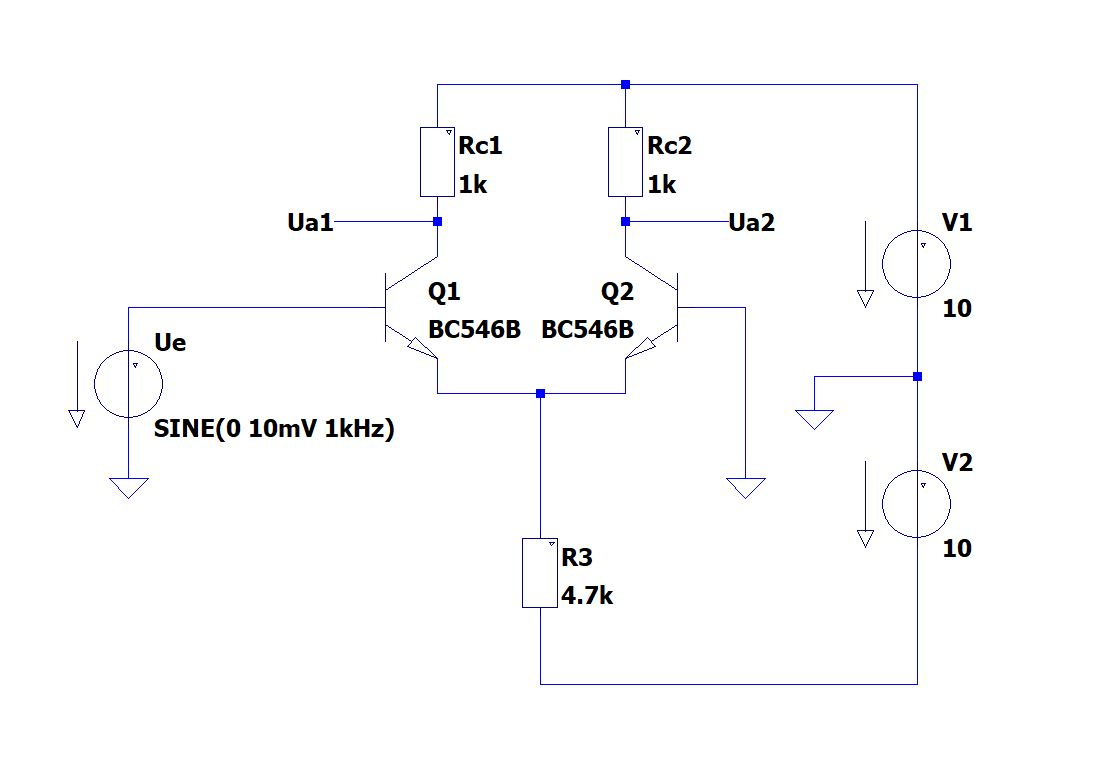
\includegraphics[scale=0.4] {../assets/images/EL2P1/Aufbau 3.1.JPG}
    \caption{Versuchsaufbau des Netzwerkes}
  \end{center}
\end{figure}



\subsection{Gegentaktverstärkung}
Um die reine Wechselspannung darstellen zulassen, werden die Gleichanteile der Spannung subtrahiert.
Im Labor geschieht dies durch die Messung in AC-Kopplung. In LTSpice könnte dafür entweder ein in Reihe geschalteter Kondensator helfen
oder es wird wie eben genannt der Mittelwert subtrahiert.

\begin{figure}[h]
  \begin{center}
    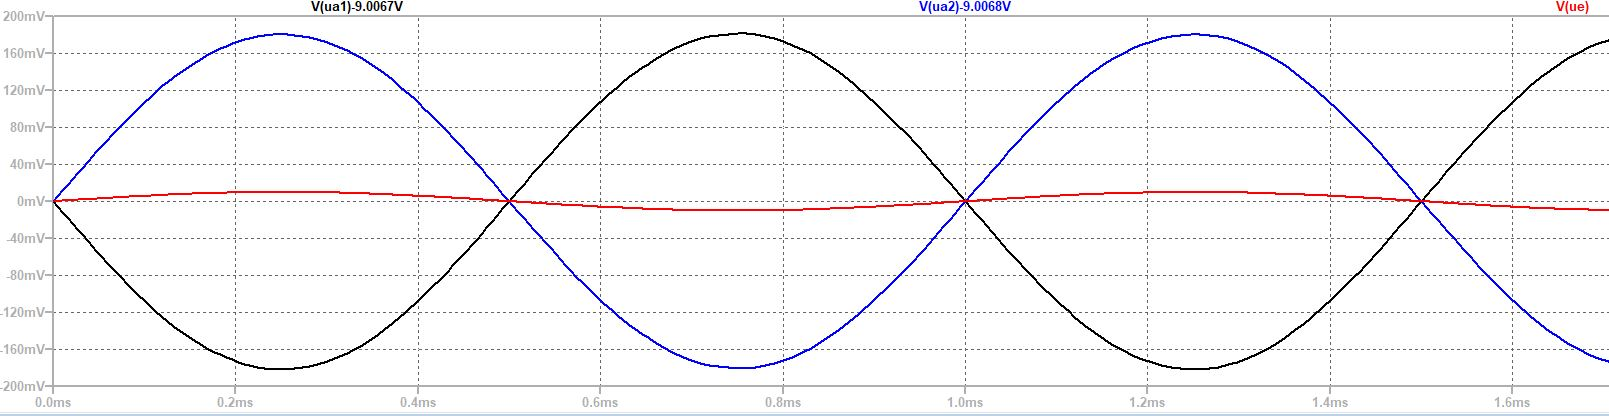
\includegraphics[scale=0.35]{../assets/images/EL2P1/Messung 3.1 Ausgang.JPG}
    \caption{Ein- und Ausgangsspannung}
  \end{center}
\end{figure}
\newpage
\subsection{Gleichtaktverstärkung}
Nun werden die Basen der Transistoren miteinander verbunden. Dabei wird die Eingangsspannung soweit erhöht bis die gleiche Ausgangsspannung wie beim Vorversuch erreicht wird.
Die ermittelte Eingangsspannung liegt hier bei $\hat{u_e} = 1,7V$.

\begin{figure}[h]
  \begin{center}
    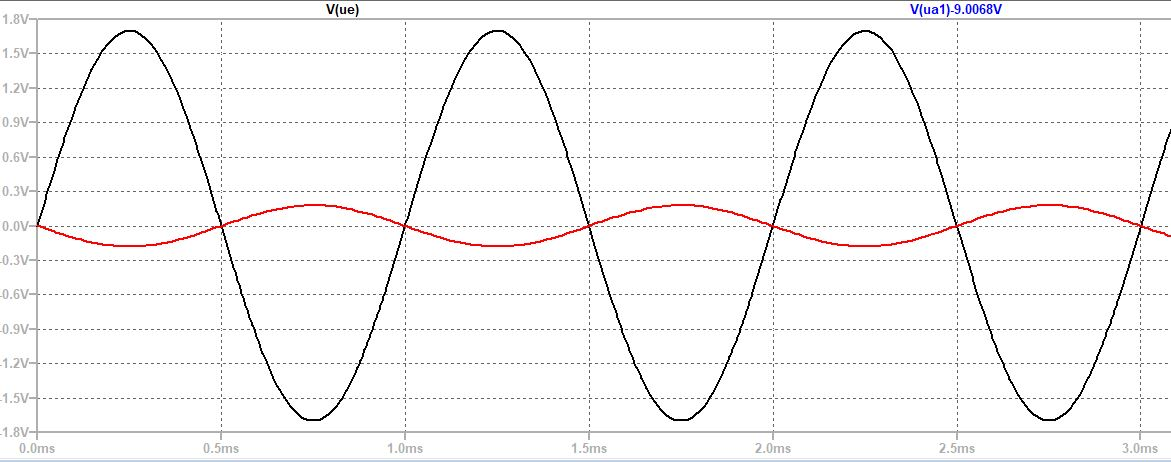
\includegraphics[scale=0.5]{../assets/images/EL2P1/Messung 3.2.JPG}
    \caption{Ein- und Ausgangsspannung}
  \end{center}
\end{figure}

Die Ausgangsspannungen liegen nun genau übereinander, weshalb nur ein Signal erkennbar ist. Dies war zu erwarten, da die Basen miteinander
verbunden sind und damit der Kollektorstrom gleich gesteuert wird.

\subsection{Auswertung der Gegen- und Gleichtaktverstärkung}
\subsubsection{Gegentaktverstärkung}

Aus den Messwerten werden die beiden Gleichtaktverstärkungen $v_{u_d1}$ und $v_{u_d2}$ bestimmt:
\begin{align*}
  v_{u_d1} = -\frac{u_{a1}}{u_e} = -\frac{180mV}{10mV} = -18\\
  v_{u_d2} = \frac{u_{a2}}{u_e} = -\frac{180mV}{10mV} = 18
\end{align*}


Vergleich der berechneten Gegentaktverstärkung $v_{u_d1}$ und $v_{u_d2}$ aus der Steilheit:

\begin{align*}
  v_{u_d1} &= - \frac{1}{2} \cdot S \cdot R_C = -\frac{1}{2} \cdot 0,038\frac{A}{V} \cdot 1k\Omega = -19 \\
  v_{u_d2} &= + \frac{1}{2} \cdot S \cdot R_C = -\frac{1}{2} \cdot 0,038\frac{A}{V} \cdot 1k\Omega = 19
\end{align*}

\subsubsection{Gleichtaktverstärkung}
Nun wird aus den Messungen die Gleichtaktverstärkung $v_{u_{gl}1}$ und $v_{u_{gl}2}$ bestimmt:

\begin{align*}
  v_{u_{gl}1} &= -\frac{u_{a1}}{u_e} = -\frac{180mV}{1,7V} = -0,105\\
  v_{u_{gl}2} &= \frac{u_{a2}}{u_e} = -\frac{180mV}{1,7V} = 0,105
\end{align*}

Nach der theoretischen Berechnung sollten folgende Werte sich ergeben:

\begin{align*}
  v_{u_{gl}1} &= -\frac{R_C}{2\cdot R_E} = -\frac{1k\Omega}{2\cdot 4,7k\Omega} = -0,106\\
  v_{u_{gl}2} &= -\frac{R_C}{2\cdot R_E} = -\frac{1k\Omega}{2\cdot 4,7k\Omega} = -0,106
\end{align*}

Auch hier gibt es minimale Abweichung, die darauf zurückzuführen sind, dass unsere Ansätze bei der Berechnung immer vereinfachte Rechnungen sind, so wird beispielsweise der Early-Effekt vernachlässigt.
LTSpice jedoch arbeitet mit sehr genauen numerischen Verfahren, so dass die Messergebnisse von den berechneten Werten abweichen können.

\subsection{Gleichtaktunterdrückung}

Aus den Messwerten ergibt sich eine Gleichtaktunterdrückung von:

\begin{align*}
  \mathrm{CMRR}_1 &= G = |\frac{v_{u_d}i}{v_{u_{gl}}}| = S \cdot R_E = 0,038 \frac{A}{V}\cdot 4,7k\Omega = 178,6 \\
  \mathrm{CMRR}_2 &= G = |\frac{v_{u_d}i}{v_{u_{gl}}}| = S \cdot R_E = 0,038 \frac{A}{V}\cdot 4,7k\Omega = 178,6
 \end{align*}

Theoretisch soll die Gleichtaktunterdrückung bei folgenden Werten liegen:

\begin{align*}
  \mathrm{CMRR}_1 &= G = |\frac{v_{u_d}i}{v_{u_{gl}}}| = \frac{18}{0,105} = 169,8\\
  \mathrm{CMRR}_2 &= G = |\frac{v_{u_d}i}{v_{u_{gl}}}| = \frac{18}{0,105} = 169,8
\end{align*}

\newpage

\section{Wechselspannungsverstärker}

\begin{task}
  TIn dieser Aufgabe wollen wir die Wechselspannungsverstärkung, die dem Differenzverstärker zugrunde liegt untersuchen.
\end{task}

\begin{figure}[h]
  \centering
  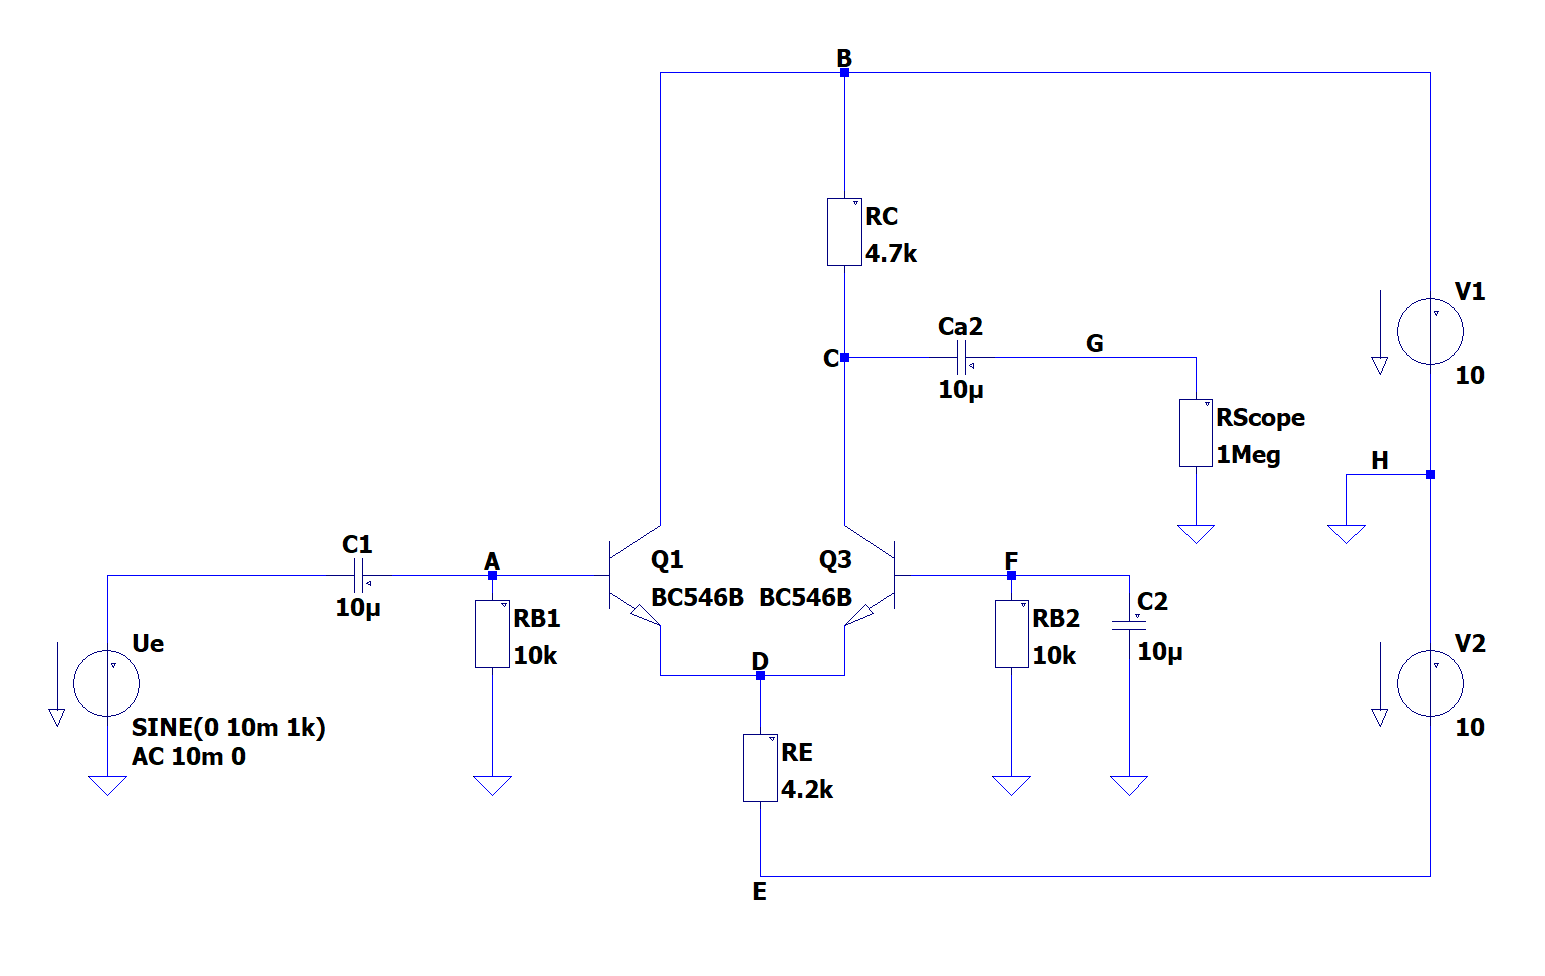
\includegraphics[scale=0.5]{../assets/images/EL2P1/abb1.png}
  \caption{Schaltplan für den Versuchsaufbau}
  \label{fig:schalt3}
\end{figure}

\subsection*{Vorbereitung}

Aus der gegebenen Spannungsverstärkung von ca. $40\mathrm{dB}$ errechnen wir nun den Emitterwiderstand $R_{E}$:
\begin{equation}
  \label{eq:1}
  v_{u} = \frac{1}{2} \cdot S \cdot R_{C} = 40 \mathrm{dB} = 100 \text{mit} S = \frac{I_{C_{0}}}{U_{T}}
\end{equation}

Und damit erkennen wir, dass:
\begin{equation}
  \label{eq:2}
  100 = \frac{I_{C_{0}}\cdot R_{C}}{2\cdot U_{T}}
\end{equation}

Wir wollen nun zunächst den Wert für $I_{C_{0}}$ berechnen:
\begin{equation}
  \label{eq:3}
  I_{C_{0}} = \frac{100\cdot 2\cdot U_{T}}{R_{C}} = \frac{100 \cdot 2 \cdot 26\mathrm{mV}}{47k\Omega} = 1,1\mathrm{mA}
\end{equation}

Wir stellen nun die betreffende Masche auf, um den Widerstandswert von $R_{E}$ zu berechnen und erhalten:
\begin{equation}
  \label{eq:4}
  0\mathrm{V} = U_{BE} - U_{B} + R_{E}\cdot I_{0}
\end{equation}

Wir stellen nun die Gleichung nach $R_{E}$ um und bekommen:
\begin{equation}
  \label{eq:5}
  R_{E} = \frac{U_{B} - U_{BE}}{I_{C_{0}}} = \frac{10\mathrm{V}-0,7\mathrm{V}}{2,2mA} = 4227\Omega.
\end{equation}

Aus der E12-Reihe wählen wir nun $2\cdot 1k\Omega$ und $1\cdot 2,2k\Omega$, womit wir auf $4,2k\Omega$ kommen.

\subsection{Simulation der Schaltung}

Wir wollen nun die Schaltung im berechneten Arbeitspunkt simulieren und die Gleichspannungspotentiale an den Punkten A-H auslesen.
\begin{table}[h]
  \centering
  \begin{tabular}[h]{|l|l|l|}
    \hline
  Messpunkt & Spannung (RMS) & Spannung (Mittelwert)\\
    \hline
  A & $35,66\mathrm{mV}$ & $-34,952\mathrm{mV}$\\
    \hline
  B & $10\mathrm{V}$ & $10\mathrm{V}$\\
    \hline
  C & $5,0215\mathrm{V}$ & $4,9793\mathrm{V}$\\
    \hline
  D & $673,4\mathrm{mV}$ & $-673,39\mathrm{mV}$\\
    \hline
  E & $10\mathrm{V}$ & $10\mathrm{V}$\\
    \hline
  F & $34,937\mathrm{mV}$ & $-34,937\mathrm{mV}$\\
    \hline
  G & $649,62\mathrm{mV}$ & $-5,7671\mathrm{mV}$\\
    \hline
    H & $0\mathrm{V}$ & $0\mathrm{V}$\\
    \hline
  \end{tabular}
  \caption{Messpunkte aus LTSpice}
  \label{tab:table1}
\end{table}

Aus den oben stehenden Messwerten werden wir nun die Basisströme, Kollektorströme und ihre Stromverstärkung berechnen:

\begin{align*}
  I_{C_{2}} &= \frac{B-C}{R_{C}} = \frac{10\mathrm{V}-4,98\mathrm{V}}{4,7k\Omega} = 1,068\mathrm{mA}\\
  I_{0} &= \frac{D-E}{R_{E}} = \frac{-0,673\mathrm{V}+10\mathrm{V}}{4,2k\Omega} = 2,22\mathrm{mA}\\
  I_{C_{1}} &= I_{0}-I_{C_{2}} = 2,22\mathrm{mA}-1,068\mathrm{mA} = 1,152\mathrm{mA}\\
  I_{B_{1}} &= \frac{A}{R_{B_{1}}} = \frac{0,035\mathrm{V}}{10k\Omega} = 3,5\mu\mathrm{A}\\
  I_{B_{2}} &= \frac{F}{R_{B_{2}}} = \frac{0,035\mathrm{V}}{10k\Omega} = 3,5\mu\mathrm{A}\\
  B_{1} &= \frac{I_{C_{1}}}{I_{B_{1}}} = \frac{1,152\mathrm{mA}}{3,5\mu\mathrm{A}} = 329,1\\
  B_{2} &= \frac{I_{C_{2}}}{I_{B_{2}}} = \frac{1,068\mathrm{mA}}{3,5\mu\mathrm{A}} = 305,1\\
\end{align*}

Die berechneten Ströme stimmen sehr genau mit den Strömen, die LTSpice berechnet überein:
\begin{figure}[h]
  \centering
  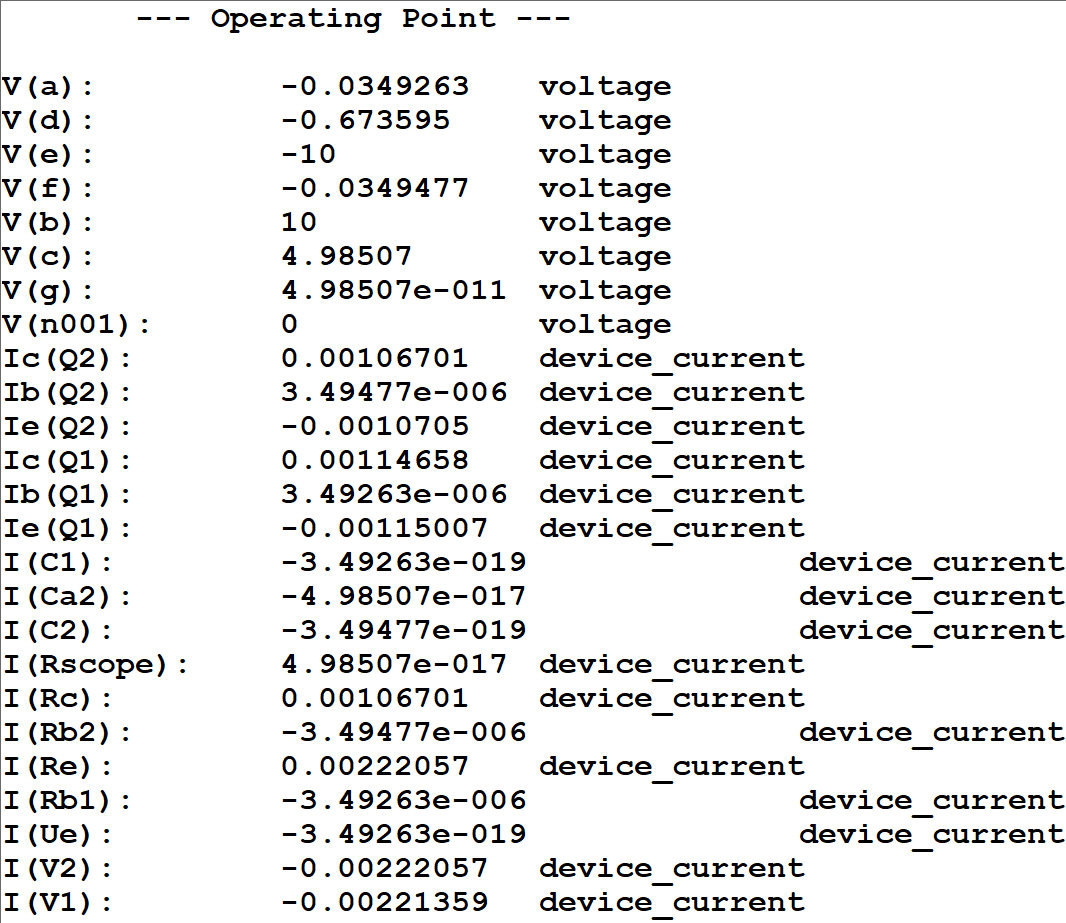
\includegraphics[scale=0.35]{../assets/images/EL2P1/abb2.png}
  \caption{Messwerte aus LTSpice}
  \label{fig:table1}
\end{figure}

\newpage
\subsection{Simulation Wechselspannungsverstärkung}

In der nächsten Teilaufgabe wollen wir nun eine Simulation mit $\hat{u}_{e} = 10\mathrm{mV}$ und $f = 1\mathrm{kHz}$ machen und dann die Wechselspannungsverstärkung ermitteln. Diese wollen wir dann mit der theoretischen Wechselspannungsverstärkung vergleichen.\\

\begin{figure}[h]
  \centering
  \begin{subfigure}[h]{0.3\textwidth}
    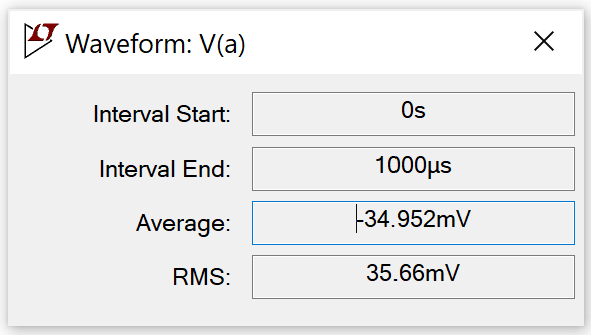
\includegraphics[width=\textwidth]{../assets/images/EL2P1/abb3.png}
    \caption{Eingangsspannung $u_{e}$}
  \end{subfigure}
  \hfill
  \begin{subfigure}[h]{0.3\textwidth}
    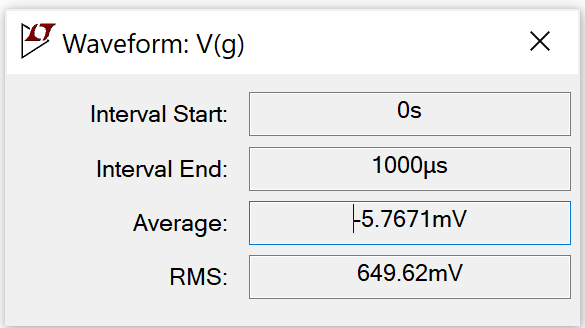
\includegraphics[width=\textwidth]{../assets/images/EL2P1/abb4.png}
    \caption{Ausgangsspannung $u_{a}$}
  \end{subfigure}
  \caption{Messwerte aus der Simulation}
  \label{fig:subfig1}
\end{figure}


Wir berechnen zunächst einmal den Wert aus der Simulation:
\begin{equation}
  \label{eq:7}
  u_{~} = \sqrt{u^{2}_{EFF} - u^{2}_{-}}
\end{equation}

\begin{equation*}
  u_{e~} = \sqrt{(35,66\mathrm{mV})^{2}-(-34,952\mathrm{mV})^{2}} = 7,07\mathrm{mV}
\end{equation*}
\begin{equation*}
  u_{a~} = \sqrt{(649,62\mathrm{mV})^{2}-(-5,7671\mathrm{mV})^{2}} = 649,59\mathrm{mV}
\end{equation*}

Nun errechnen wir aus den beiden oberen Werten die Wechselspannungsverstärkung:

\begin{equation}
  \label{eq:6}
  v_{u} = \frac{u_{a~}}{u_{e~}} = \frac{649,59\mathrm{mV}}{7,07\mathrm{mV}} = 91,88.
\end{equation}

Wir erkennen, dass dieser Wert nicht extrem weit weg von unserem angestrebten Wert von 100 liegt. Abweichungen können sowohl durch Rundungen, Bauteilabweichungen/-ungenauigkeiten oder durch numerische Verfahren entstehen.

\subsection{Eingangswiderstand der Schaltung}

\begin{figure}[h]
  \centering
  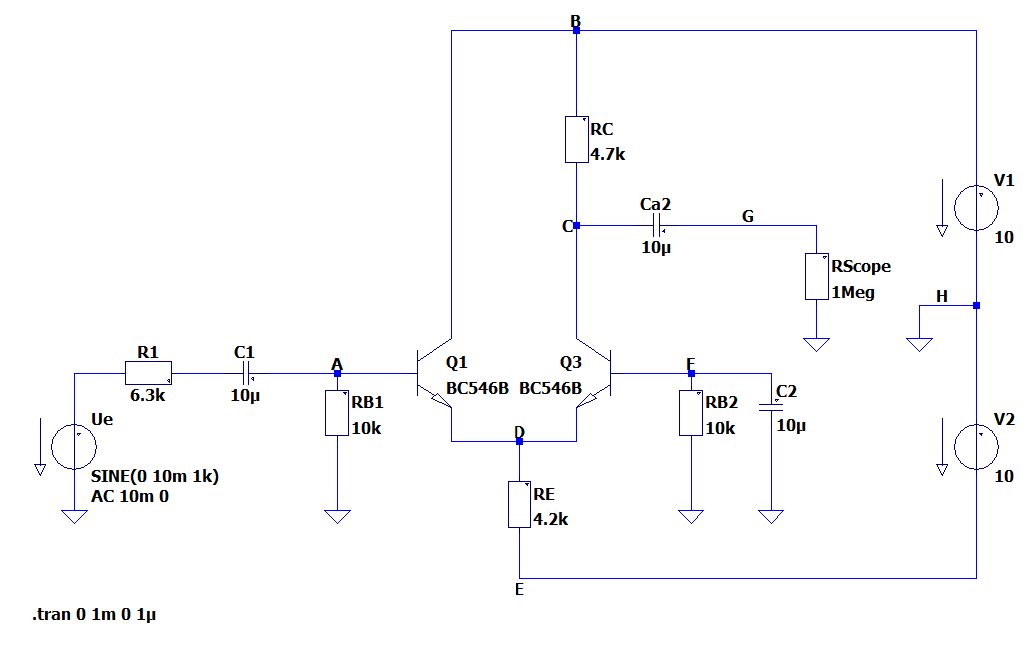
\includegraphics[width=\textwidth]{../assets/images/EL2P1/abb5.png}
  \caption{Schaltplan für die Messung 4.3}
  \label{fig:input}
\end{figure}

Im nächsten Teilversuch vergleichen wir den Eingangswiderstand der Schaltung, den wir mithilfe einer Formel aus der Vorlesung berechnen können und dem Eingangswiderstand der Schaltung, die wir mittels der Halbausschlagsmethode ermitteln können.

Dazu berechnen wir zuerst einmal den Eingangswiderstand über:

\begin{equation}
  \label{eq:8}
  r_{ein} = R_{B}||(2\cdot r_{BE})
\end{equation}

\begin{equation*}
  \label{eq:9}
  \frac{R_{B}\cdot 2\cdot r_{BE}}{R_{B}+2\cdot r_{BE}} = \frac{10k\Omega \cdot 2 \cdot 4,2k\Omega}{10k\Omega + 2\cdot 4,2k\Omega} = 4,565k\Omega
\end{equation*}
\newpage
Wir wollen nun die Halbausschlagmethode nutzen, um einen entsprechenden Vergleichswert zu bekommen:

\begin{figure}[h]
  \centering
  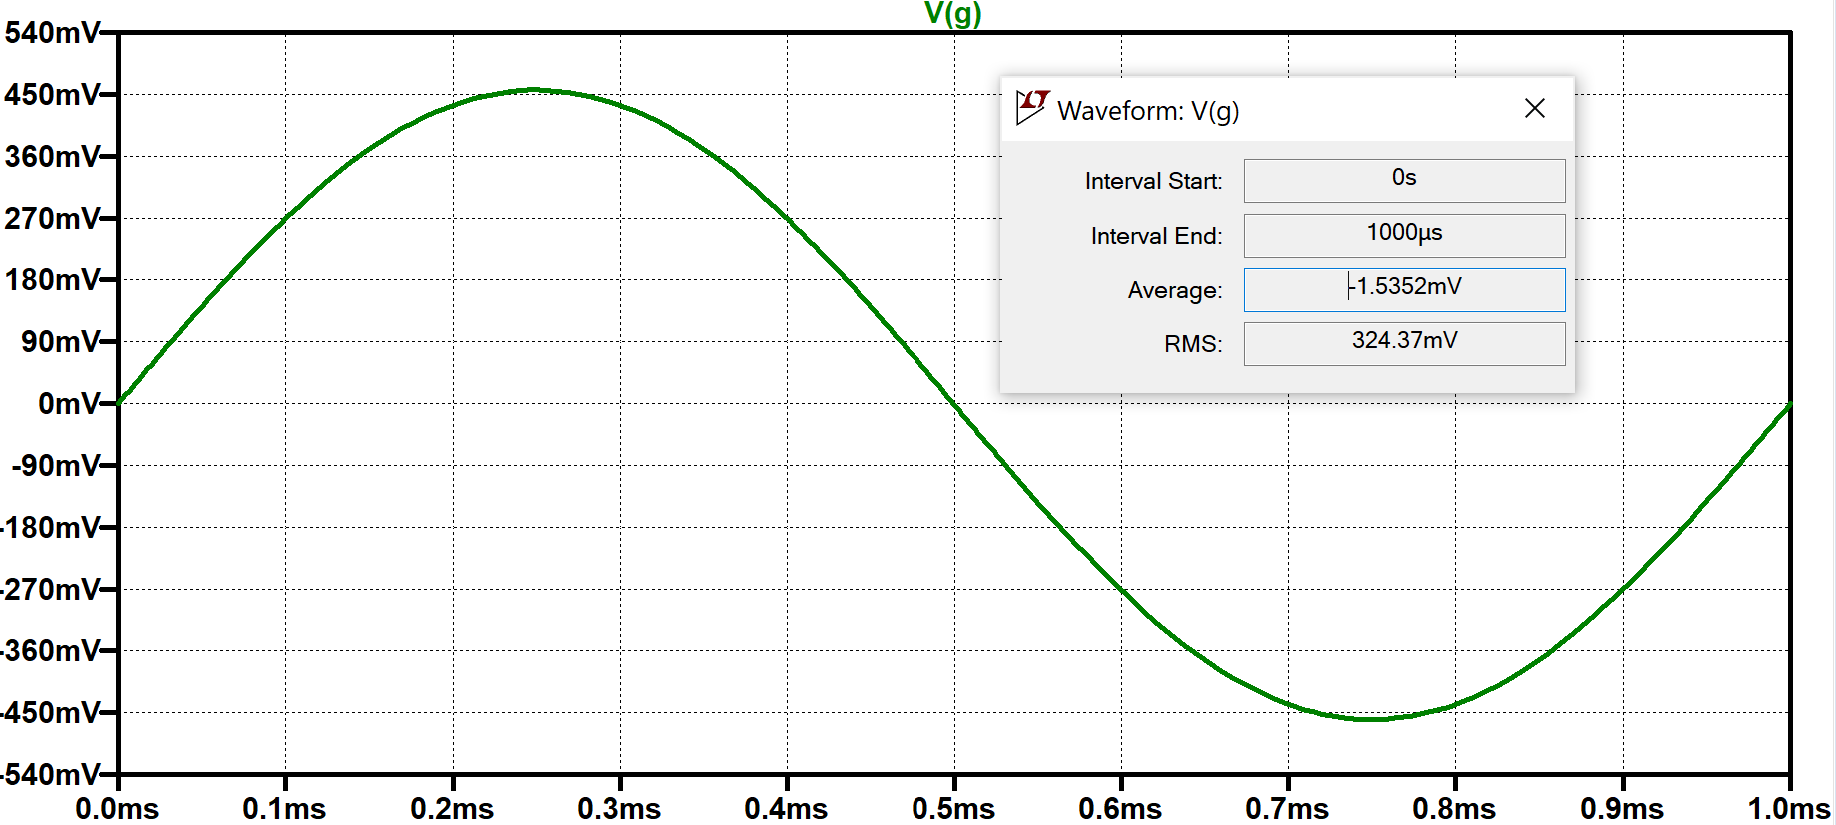
\includegraphics[width=\textwidth]{../assets/images/EL2P1/abb6.png}
  \caption{Messung für 4.3}
  \label{fig:input2}
\end{figure}

Wir erkennen, dass der Wert aus der Simulation erhöht ist und etwa $6,3k\Omega$ beträgt.
\newpage
\subsection{Ausgangswiderstand der Schaltung}

\begin{figure}[h]
  \centering
  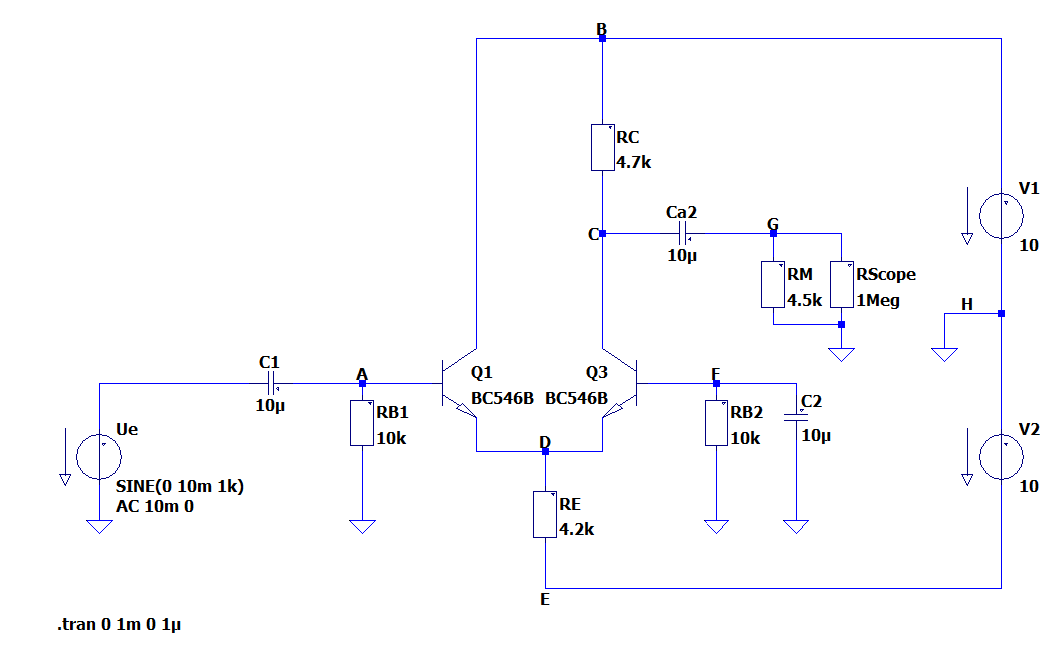
\includegraphics[width=\textwidth]{../assets/images/EL2P1/abb7.png}
  \caption{Aufbau der Schaltung für 4.4}
  \label{fig:schalt44}
\end{figure}

Im vorletzten Versuch wiederholen wir nun den vorigen Vorgang, wobei wir uns hier jedoch auf den Ausgangswiderstand beziehen. Wir wollen also wieder zunächst den Ausgangswiderstand theoretisch beschreiben und ihn dann mithilfe der Simulation praktisch ermitteln:

\begin{equation*}
  r_{aus}\approx R_{C} = 4,7k\Omega
\end{equation*}

\begin{figure}[h]
  \centering
  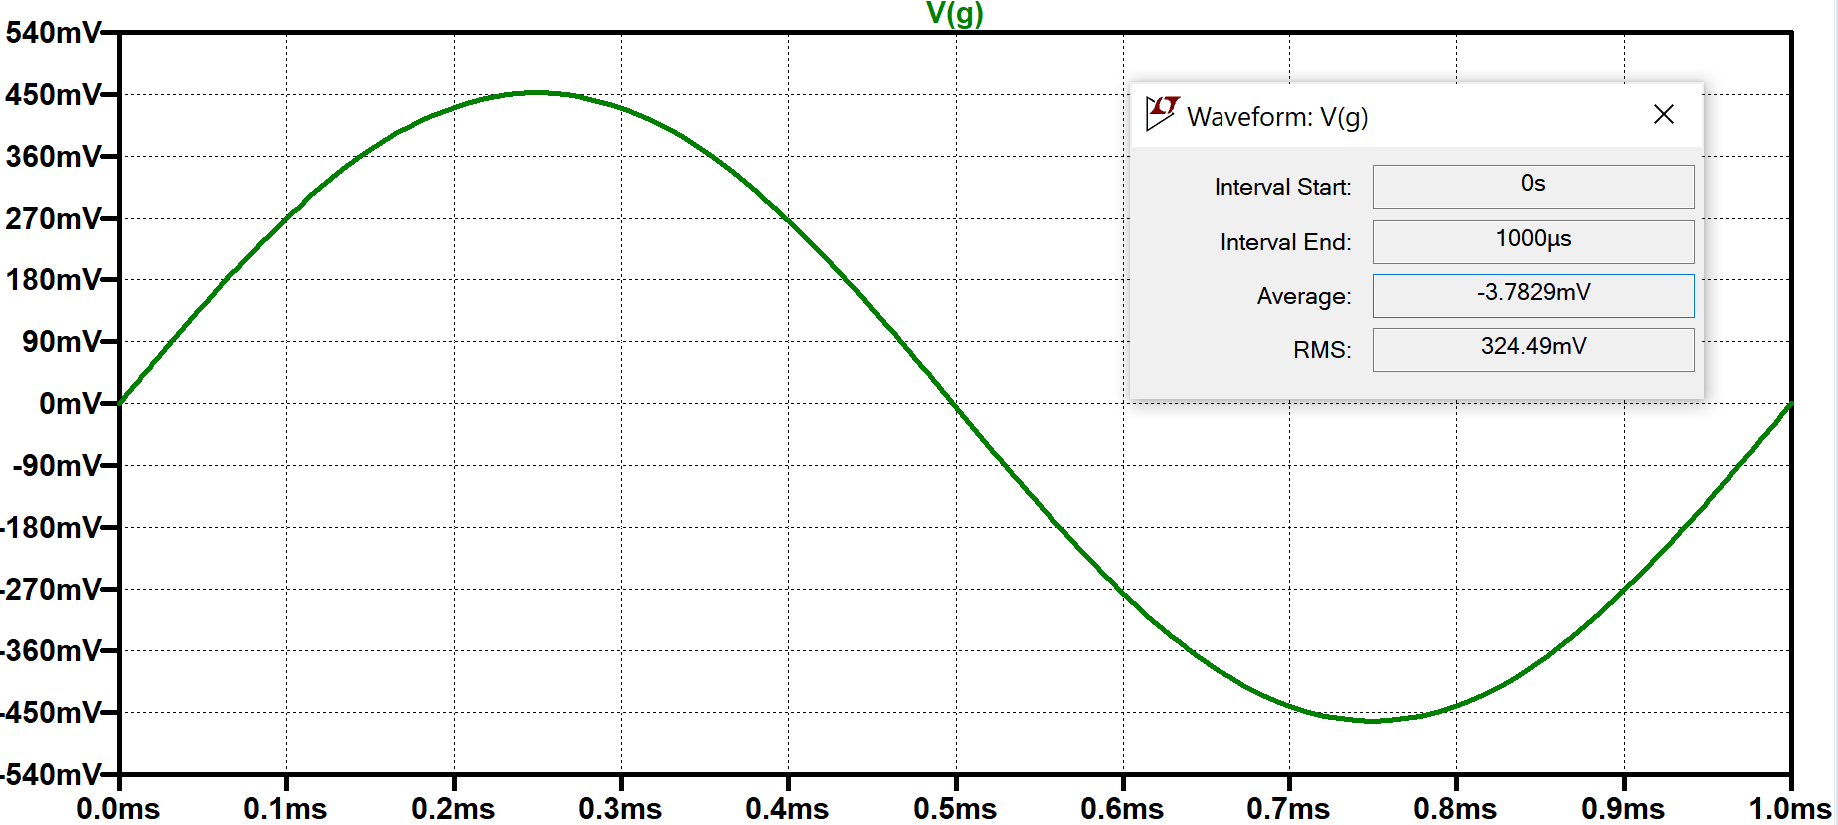
\includegraphics[width=\textwidth]{../assets/images/EL2P1/abb8.png}
  \caption{Messung für 4.4}
  \label{fig:diag44}
\end{figure}
\newpage
Mit der Simulation ermitteln wir dann allerdings einen Wert von ca. $4,5k\Omega$. Dieser Wert ist nur leicht geringer als erwartet und entspricht im Groben den Erwartungen.\\
In beiden Versuchen haben wir die Halbsspannungsmethode verwendet. Wir ermitteln damit, welchen Ein- bzw. Ausgangswiderstand die Schaltung hat. Dabei erhöhen wir unseren Messwiderstand $R_{M}$ solange, bis ungefähr die Hälfte der Spannung über unseren $R_{M}$ abfällt. Der $R_{M}$ hat dann den gleichen Spannungswert wie unser gesuchter Widerstand, weil sich dann die Spannung über beide Widerstände, die dann in Reihe sind, gleichmäßig im Verhältnis 1:1 aufteilt. Wir wissen nämlich, aus dem Ohm'schen Gesetz, dass wenn wir $U = R \cdot I$ nehmen, und Spannung $U$ und Strom $I$, denn die Widerstände sind in Reihe, gleich sind, auch der Widerstandswert $R$ für beide Widerstände identisch sein muss.
\newpage
\subsection{AC-Analyse der Schaltung}

Wir führen im letzten Schritt eine AC-Analyse im Bereich $f=10\mathrm{Hz}...10\mathrm{MHz}$ durch und stellen den Vorgang als Graph nach Frequenz und Spannungsverstärkung in halblogarithmischer Skalierung dar:

\begin{figure}[h]
  \centering
  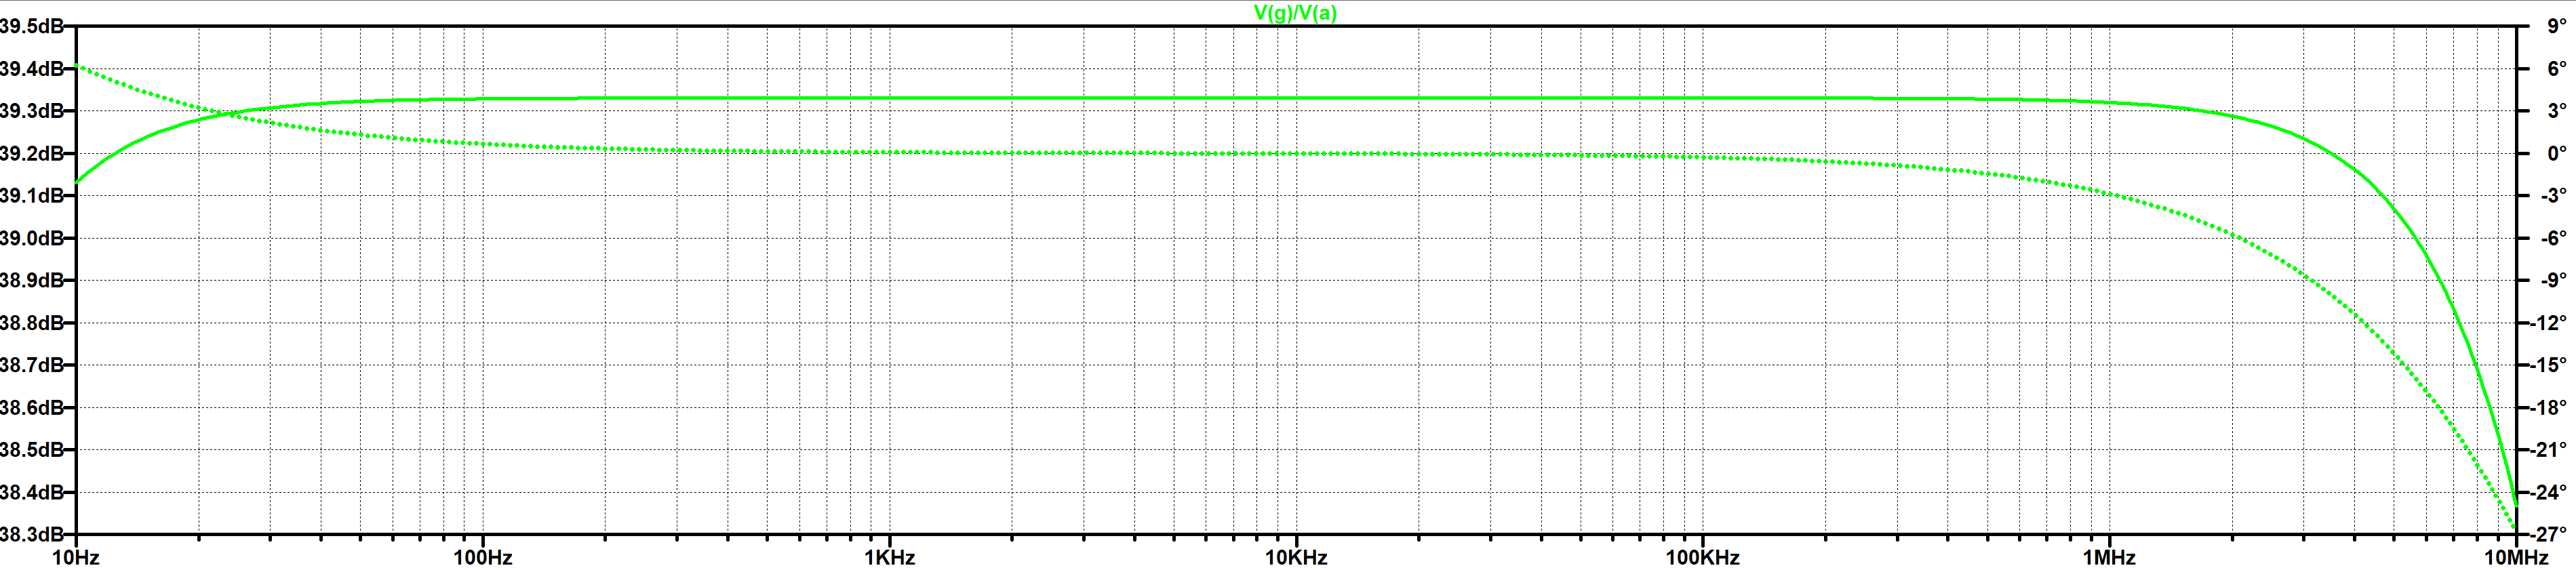
\includegraphics[width=\textwidth]{../assets/images/EL2P1/abb9.png}
  \caption{Messung der AC-Analyse}
  \label{fig:ac}
\end{figure}

\bibliographystyle{plain}
\bibliography{ELP2_1}{}
\end{document}
